\input{tikz}
\begin{document}
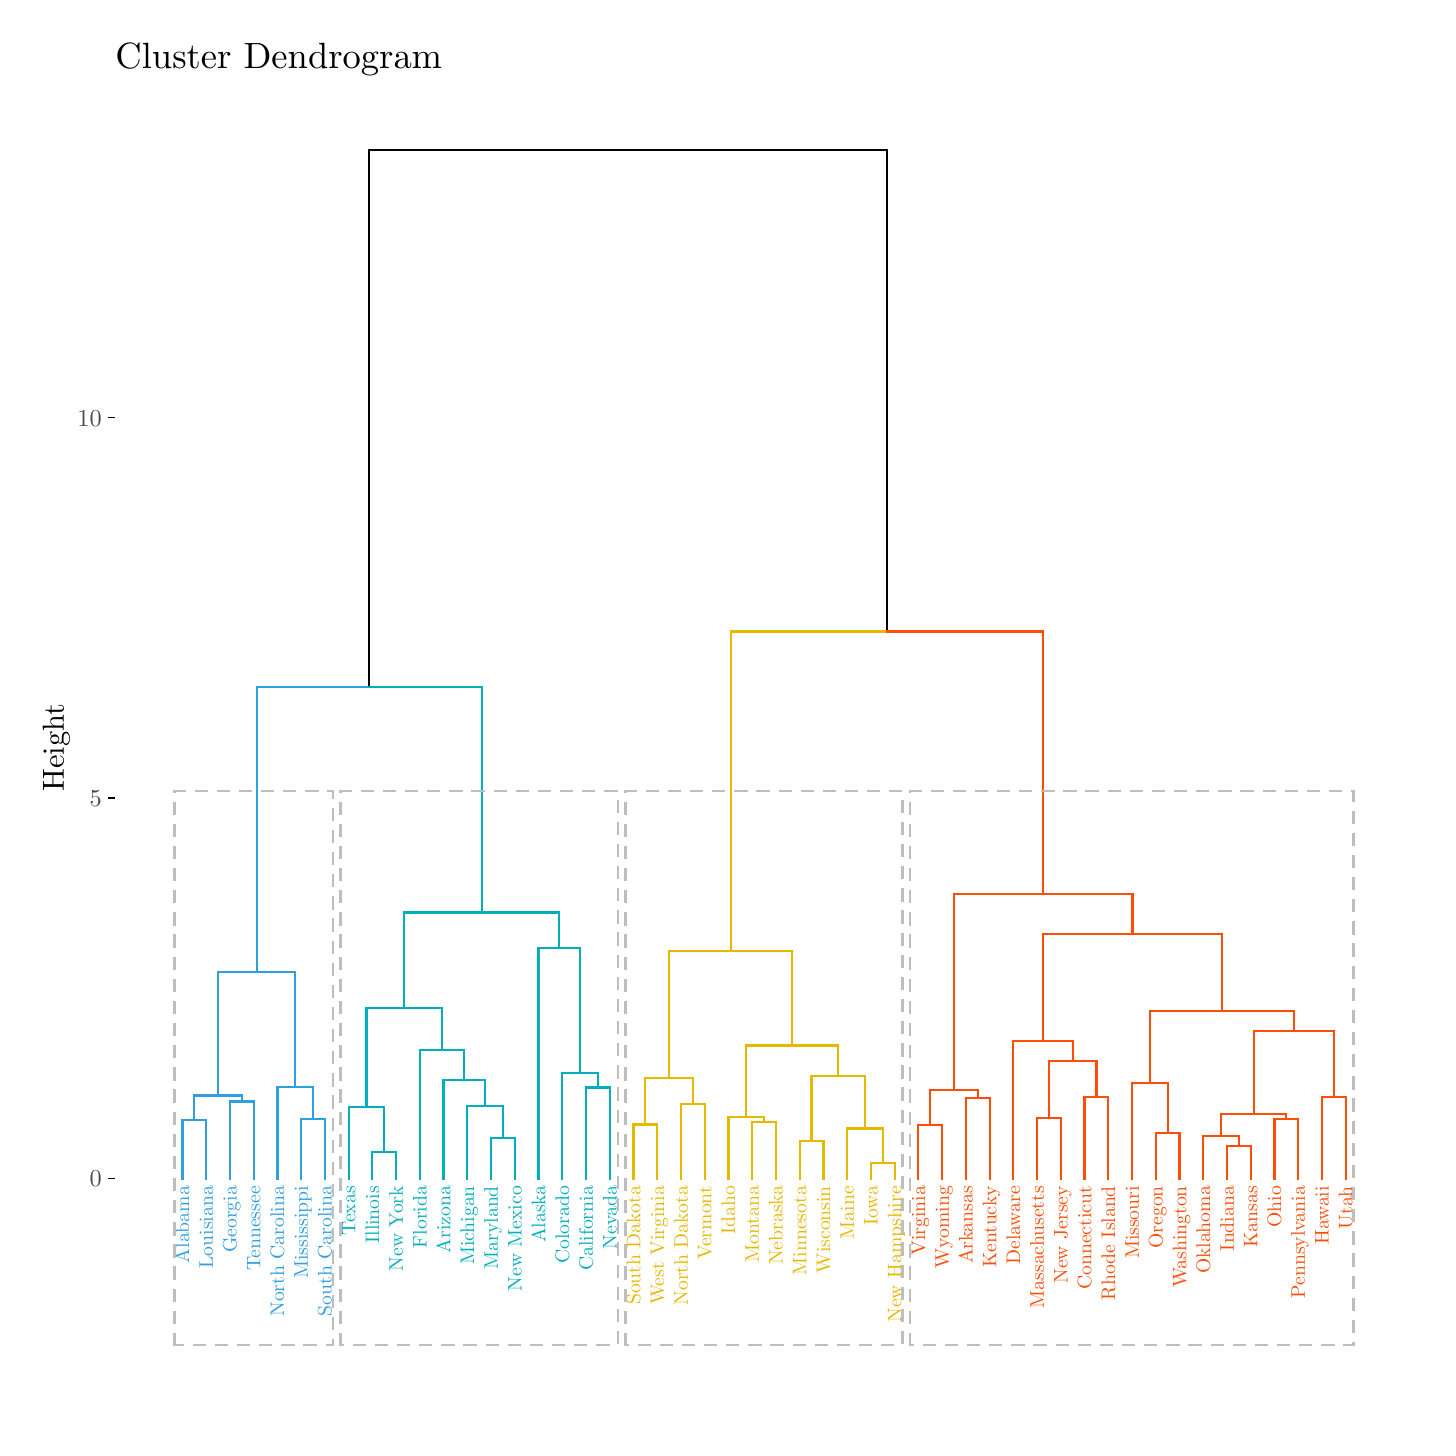
\begin{tikzpicture}[x=1pt,y=1pt]


\definecolor{fillColor}{RGB}{255,255,255}
\path[use as bounding box,fill=fillColor,fill opacity=0.00] (0,0) rectangle (505.89,505.89);
\begin{scope}
\path[clip] (  0.00,  0.00) rectangle (505.89,505.89);
\definecolor{drawColor}{RGB}{255,255,255}
\definecolor{fillColor}{RGB}{255,255,255}

\path[draw=drawColor,line width= 0.6pt,line join=round,line cap=round,fill=fillColor] (  0.00,  0.00) rectangle (505.89,505.89);
\end{scope}
\begin{scope}
\path[clip] ( 31.71,  8.25) rectangle (500.39,483.23);
\definecolor{fillColor}{RGB}{255,255,255}

\path[fill=fillColor] ( 31.71,  8.25) rectangle (500.39,483.23);
\definecolor{drawColor}{RGB}{0,0,0}

\path[draw=drawColor,line width= 0.8pt,line join=round,line cap=rect] (216.95,461.64) -- (123.42,461.64);

\path[draw=drawColor,line width= 0.8pt,line join=round,line cap=rect] (123.42,461.64) -- (123.42,267.70);
\definecolor{drawColor}{RGB}{46,159,223}

\path[draw=drawColor,line width= 0.8pt,line join=round,line cap=rect] (123.42,267.70) -- ( 82.74,267.70);

\path[draw=drawColor,line width= 0.8pt,line join=round,line cap=rect] ( 82.74,267.70) -- ( 82.74,164.67);

\path[draw=drawColor,line width= 0.8pt,line join=round,line cap=rect] ( 82.74,164.67) -- ( 68.80,164.67);

\path[draw=drawColor,line width= 0.8pt,line join=round,line cap=rect] ( 68.80,164.67) -- ( 68.80,120.04);

\path[draw=drawColor,line width= 0.8pt,line join=round,line cap=rect] ( 68.80,120.04) -- ( 60.22,120.04);

\path[draw=drawColor,line width= 0.8pt,line join=round,line cap=rect] ( 60.22,120.04) -- ( 60.22,111.27);

\path[draw=drawColor,line width= 0.8pt,line join=round,line cap=rect] ( 60.22,111.27) -- ( 55.93,111.27);

\path[draw=drawColor,line width= 0.8pt,line join=round,line cap=rect] ( 55.93,111.27) -- ( 55.93, 90.04);

\path[draw=drawColor,line width= 0.8pt,line join=round,line cap=rect] ( 60.22,111.27) -- ( 64.51,111.27);

\path[draw=drawColor,line width= 0.8pt,line join=round,line cap=rect] ( 64.51,111.27) -- ( 64.51, 90.04);

\path[draw=drawColor,line width= 0.8pt,line join=round,line cap=rect] ( 68.80,120.04) -- ( 77.38,120.04);

\path[draw=drawColor,line width= 0.8pt,line join=round,line cap=rect] ( 77.38,120.04) -- ( 77.38,117.87);

\path[draw=drawColor,line width= 0.8pt,line join=round,line cap=rect] ( 77.38,117.87) -- ( 73.09,117.87);

\path[draw=drawColor,line width= 0.8pt,line join=round,line cap=rect] ( 73.09,117.87) -- ( 73.09, 90.04);

\path[draw=drawColor,line width= 0.8pt,line join=round,line cap=rect] ( 77.38,117.87) -- ( 81.67,117.87);

\path[draw=drawColor,line width= 0.8pt,line join=round,line cap=rect] ( 81.67,117.87) -- ( 81.67, 90.04);

\path[draw=drawColor,line width= 0.8pt,line join=round,line cap=rect] ( 82.74,164.67) -- ( 96.68,164.67);

\path[draw=drawColor,line width= 0.8pt,line join=round,line cap=rect] ( 96.68,164.67) -- ( 96.68,123.23);

\path[draw=drawColor,line width= 0.8pt,line join=round,line cap=rect] ( 96.68,123.23) -- ( 90.24,123.23);

\path[draw=drawColor,line width= 0.8pt,line join=round,line cap=rect] ( 90.24,123.23) -- ( 90.24, 90.04);

\path[draw=drawColor,line width= 0.8pt,line join=round,line cap=rect] ( 96.68,123.23) -- (103.11,123.23);

\path[draw=drawColor,line width= 0.8pt,line join=round,line cap=rect] (103.11,123.23) -- (103.11,111.66);

\path[draw=drawColor,line width= 0.8pt,line join=round,line cap=rect] (103.11,111.66) -- ( 98.82,111.66);

\path[draw=drawColor,line width= 0.8pt,line join=round,line cap=rect] ( 98.82,111.66) -- ( 98.82, 90.04);

\path[draw=drawColor,line width= 0.8pt,line join=round,line cap=rect] (103.11,111.66) -- (107.40,111.66);

\path[draw=drawColor,line width= 0.8pt,line join=round,line cap=rect] (107.40,111.66) -- (107.40, 90.04);
\definecolor{drawColor}{RGB}{0,175,187}

\path[draw=drawColor,line width= 0.8pt,line join=round,line cap=rect] (123.42,267.70) -- (164.10,267.70);

\path[draw=drawColor,line width= 0.8pt,line join=round,line cap=rect] (164.10,267.70) -- (164.10,186.16);

\path[draw=drawColor,line width= 0.8pt,line join=round,line cap=rect] (164.10,186.16) -- (136.08,186.16);

\path[draw=drawColor,line width= 0.8pt,line join=round,line cap=rect] (136.08,186.16) -- (136.08,151.68);

\path[draw=drawColor,line width= 0.8pt,line join=round,line cap=rect] (136.08,151.68) -- (122.41,151.68);

\path[draw=drawColor,line width= 0.8pt,line join=round,line cap=rect] (122.41,151.68) -- (122.41,115.96);

\path[draw=drawColor,line width= 0.8pt,line join=round,line cap=rect] (122.41,115.96) -- (115.98,115.96);

\path[draw=drawColor,line width= 0.8pt,line join=round,line cap=rect] (115.98,115.96) -- (115.98, 90.04);

\path[draw=drawColor,line width= 0.8pt,line join=round,line cap=rect] (122.41,115.96) -- (128.85,115.96);

\path[draw=drawColor,line width= 0.8pt,line join=round,line cap=rect] (128.85,115.96) -- (128.85, 99.67);

\path[draw=drawColor,line width= 0.8pt,line join=round,line cap=rect] (128.85, 99.67) -- (124.56, 99.67);

\path[draw=drawColor,line width= 0.8pt,line join=round,line cap=rect] (124.56, 99.67) -- (124.56, 90.04);

\path[draw=drawColor,line width= 0.8pt,line join=round,line cap=rect] (128.85, 99.67) -- (133.13, 99.67);

\path[draw=drawColor,line width= 0.8pt,line join=round,line cap=rect] (133.13, 99.67) -- (133.13, 90.04);

\path[draw=drawColor,line width= 0.8pt,line join=round,line cap=rect] (136.08,151.68) -- (149.75,151.68);

\path[draw=drawColor,line width= 0.8pt,line join=round,line cap=rect] (149.75,151.68) -- (149.75,136.52);

\path[draw=drawColor,line width= 0.8pt,line join=round,line cap=rect] (149.75,136.52) -- (141.71,136.52);

\path[draw=drawColor,line width= 0.8pt,line join=round,line cap=rect] (141.71,136.52) -- (141.71, 90.04);

\path[draw=drawColor,line width= 0.8pt,line join=round,line cap=rect] (149.75,136.52) -- (157.80,136.52);

\path[draw=drawColor,line width= 0.8pt,line join=round,line cap=rect] (157.80,136.52) -- (157.80,125.75);

\path[draw=drawColor,line width= 0.8pt,line join=round,line cap=rect] (157.80,125.75) -- (150.29,125.75);

\path[draw=drawColor,line width= 0.8pt,line join=round,line cap=rect] (150.29,125.75) -- (150.29, 90.04);

\path[draw=drawColor,line width= 0.8pt,line join=round,line cap=rect] (157.80,125.75) -- (165.30,125.75);

\path[draw=drawColor,line width= 0.8pt,line join=round,line cap=rect] (165.30,125.75) -- (165.30,116.19);

\path[draw=drawColor,line width= 0.8pt,line join=round,line cap=rect] (165.30,116.19) -- (158.87,116.19);

\path[draw=drawColor,line width= 0.8pt,line join=round,line cap=rect] (158.87,116.19) -- (158.87, 90.04);

\path[draw=drawColor,line width= 0.8pt,line join=round,line cap=rect] (165.30,116.19) -- (171.74,116.19);

\path[draw=drawColor,line width= 0.8pt,line join=round,line cap=rect] (171.74,116.19) -- (171.74,104.76);

\path[draw=drawColor,line width= 0.8pt,line join=round,line cap=rect] (171.74,104.76) -- (167.45,104.76);

\path[draw=drawColor,line width= 0.8pt,line join=round,line cap=rect] (167.45,104.76) -- (167.45, 90.04);

\path[draw=drawColor,line width= 0.8pt,line join=round,line cap=rect] (171.74,104.76) -- (176.02,104.76);

\path[draw=drawColor,line width= 0.8pt,line join=round,line cap=rect] (176.02,104.76) -- (176.02, 90.04);

\path[draw=drawColor,line width= 0.8pt,line join=round,line cap=rect] (164.10,186.16) -- (192.11,186.16);

\path[draw=drawColor,line width= 0.8pt,line join=round,line cap=rect] (192.11,186.16) -- (192.11,173.21);

\path[draw=drawColor,line width= 0.8pt,line join=round,line cap=rect] (192.11,173.21) -- (184.60,173.21);

\path[draw=drawColor,line width= 0.8pt,line join=round,line cap=rect] (184.60,173.21) -- (184.60, 90.04);

\path[draw=drawColor,line width= 0.8pt,line join=round,line cap=rect] (192.11,173.21) -- (199.61,173.21);

\path[draw=drawColor,line width= 0.8pt,line join=round,line cap=rect] (199.61,173.21) -- (199.61,128.26);

\path[draw=drawColor,line width= 0.8pt,line join=round,line cap=rect] (199.61,128.26) -- (193.18,128.26);

\path[draw=drawColor,line width= 0.8pt,line join=round,line cap=rect] (193.18,128.26) -- (193.18, 90.04);

\path[draw=drawColor,line width= 0.8pt,line join=round,line cap=rect] (199.61,128.26) -- (206.05,128.26);

\path[draw=drawColor,line width= 0.8pt,line join=round,line cap=rect] (206.05,128.26) -- (206.05,122.94);

\path[draw=drawColor,line width= 0.8pt,line join=round,line cap=rect] (206.05,122.94) -- (201.76,122.94);

\path[draw=drawColor,line width= 0.8pt,line join=round,line cap=rect] (201.76,122.94) -- (201.76, 90.04);

\path[draw=drawColor,line width= 0.8pt,line join=round,line cap=rect] (206.05,122.94) -- (210.34,122.94);

\path[draw=drawColor,line width= 0.8pt,line join=round,line cap=rect] (210.34,122.94) -- (210.34, 90.04);
\definecolor{drawColor}{RGB}{0,0,0}

\path[draw=drawColor,line width= 0.8pt,line join=round,line cap=rect] (216.95,461.64) -- (310.49,461.64);

\path[draw=drawColor,line width= 0.8pt,line join=round,line cap=rect] (310.49,461.64) -- (310.49,287.66);
\definecolor{drawColor}{RGB}{231,184,0}

\path[draw=drawColor,line width= 0.8pt,line join=round,line cap=rect] (310.49,287.66) -- (254.03,287.66);

\path[draw=drawColor,line width= 0.8pt,line join=round,line cap=rect] (254.03,287.66) -- (254.03,172.33);

\path[draw=drawColor,line width= 0.8pt,line join=round,line cap=rect] (254.03,172.33) -- (231.78,172.33);

\path[draw=drawColor,line width= 0.8pt,line join=round,line cap=rect] (231.78,172.33) -- (231.78,126.25);

\path[draw=drawColor,line width= 0.8pt,line join=round,line cap=rect] (231.78,126.25) -- (223.20,126.25);

\path[draw=drawColor,line width= 0.8pt,line join=round,line cap=rect] (223.20,126.25) -- (223.20,109.58);

\path[draw=drawColor,line width= 0.8pt,line join=round,line cap=rect] (223.20,109.58) -- (218.91,109.58);

\path[draw=drawColor,line width= 0.8pt,line join=round,line cap=rect] (218.91,109.58) -- (218.91, 90.04);

\path[draw=drawColor,line width= 0.8pt,line join=round,line cap=rect] (223.20,109.58) -- (227.49,109.58);

\path[draw=drawColor,line width= 0.8pt,line join=round,line cap=rect] (227.49,109.58) -- (227.49, 90.04);

\path[draw=drawColor,line width= 0.8pt,line join=round,line cap=rect] (231.78,126.25) -- (240.36,126.25);

\path[draw=drawColor,line width= 0.8pt,line join=round,line cap=rect] (240.36,126.25) -- (240.36,117.05);

\path[draw=drawColor,line width= 0.8pt,line join=round,line cap=rect] (240.36,117.05) -- (236.07,117.05);

\path[draw=drawColor,line width= 0.8pt,line join=round,line cap=rect] (236.07,117.05) -- (236.07, 90.04);

\path[draw=drawColor,line width= 0.8pt,line join=round,line cap=rect] (240.36,117.05) -- (244.65,117.05);

\path[draw=drawColor,line width= 0.8pt,line join=round,line cap=rect] (244.65,117.05) -- (244.65, 90.04);

\path[draw=drawColor,line width= 0.8pt,line join=round,line cap=rect] (254.03,172.33) -- (276.28,172.33);

\path[draw=drawColor,line width= 0.8pt,line join=round,line cap=rect] (276.28,172.33) -- (276.28,138.11);

\path[draw=drawColor,line width= 0.8pt,line join=round,line cap=rect] (276.28,138.11) -- (259.66,138.11);

\path[draw=drawColor,line width= 0.8pt,line join=round,line cap=rect] (259.66,138.11) -- (259.66,112.24);

\path[draw=drawColor,line width= 0.8pt,line join=round,line cap=rect] (259.66,112.24) -- (253.23,112.24);

\path[draw=drawColor,line width= 0.8pt,line join=round,line cap=rect] (253.23,112.24) -- (253.23, 90.04);

\path[draw=drawColor,line width= 0.8pt,line join=round,line cap=rect] (259.66,112.24) -- (266.09,112.24);

\path[draw=drawColor,line width= 0.8pt,line join=round,line cap=rect] (266.09,112.24) -- (266.09,110.35);

\path[draw=drawColor,line width= 0.8pt,line join=round,line cap=rect] (266.09,110.35) -- (261.80,110.35);

\path[draw=drawColor,line width= 0.8pt,line join=round,line cap=rect] (261.80,110.35) -- (261.80, 90.04);

\path[draw=drawColor,line width= 0.8pt,line join=round,line cap=rect] (266.09,110.35) -- (270.38,110.35);

\path[draw=drawColor,line width= 0.8pt,line join=round,line cap=rect] (270.38,110.35) -- (270.38, 90.04);

\path[draw=drawColor,line width= 0.8pt,line join=round,line cap=rect] (276.28,138.11) -- (292.90,138.11);

\path[draw=drawColor,line width= 0.8pt,line join=round,line cap=rect] (292.90,138.11) -- (292.90,127.01);

\path[draw=drawColor,line width= 0.8pt,line join=round,line cap=rect] (292.90,127.01) -- (283.25,127.01);

\path[draw=drawColor,line width= 0.8pt,line join=round,line cap=rect] (283.25,127.01) -- (283.25,103.62);

\path[draw=drawColor,line width= 0.8pt,line join=round,line cap=rect] (283.25,103.62) -- (278.96,103.62);

\path[draw=drawColor,line width= 0.8pt,line join=round,line cap=rect] (278.96,103.62) -- (278.96, 90.04);

\path[draw=drawColor,line width= 0.8pt,line join=round,line cap=rect] (283.25,103.62) -- (287.54,103.62);

\path[draw=drawColor,line width= 0.8pt,line join=round,line cap=rect] (287.54,103.62) -- (287.54, 90.04);

\path[draw=drawColor,line width= 0.8pt,line join=round,line cap=rect] (292.90,127.01) -- (302.55,127.01);

\path[draw=drawColor,line width= 0.8pt,line join=round,line cap=rect] (302.55,127.01) -- (302.55,108.07);

\path[draw=drawColor,line width= 0.8pt,line join=round,line cap=rect] (302.55,108.07) -- (296.12,108.07);

\path[draw=drawColor,line width= 0.8pt,line join=round,line cap=rect] (296.12,108.07) -- (296.12, 90.04);

\path[draw=drawColor,line width= 0.8pt,line join=round,line cap=rect] (302.55,108.07) -- (308.98,108.07);

\path[draw=drawColor,line width= 0.8pt,line join=round,line cap=rect] (308.98,108.07) -- (308.98, 95.70);

\path[draw=drawColor,line width= 0.8pt,line join=round,line cap=rect] (308.98, 95.70) -- (304.70, 95.70);

\path[draw=drawColor,line width= 0.8pt,line join=round,line cap=rect] (304.70, 95.70) -- (304.70, 90.04);

\path[draw=drawColor,line width= 0.8pt,line join=round,line cap=rect] (308.98, 95.70) -- (313.27, 95.70);

\path[draw=drawColor,line width= 0.8pt,line join=round,line cap=rect] (313.27, 95.70) -- (313.27, 90.04);
\definecolor{drawColor}{RGB}{252,78,7}

\path[draw=drawColor,line width= 0.8pt,line join=round,line cap=rect] (310.49,287.66) -- (366.95,287.66);

\path[draw=drawColor,line width= 0.8pt,line join=round,line cap=rect] (366.95,287.66) -- (366.95,192.70);

\path[draw=drawColor,line width= 0.8pt,line join=round,line cap=rect] (366.95,192.70) -- (334.72,192.70);

\path[draw=drawColor,line width= 0.8pt,line join=round,line cap=rect] (334.72,192.70) -- (334.72,121.95);

\path[draw=drawColor,line width= 0.8pt,line join=round,line cap=rect] (334.72,121.95) -- (326.14,121.95);

\path[draw=drawColor,line width= 0.8pt,line join=round,line cap=rect] (326.14,121.95) -- (326.14,109.39);

\path[draw=drawColor,line width= 0.8pt,line join=round,line cap=rect] (326.14,109.39) -- (321.85,109.39);

\path[draw=drawColor,line width= 0.8pt,line join=round,line cap=rect] (321.85,109.39) -- (321.85, 90.04);

\path[draw=drawColor,line width= 0.8pt,line join=round,line cap=rect] (326.14,109.39) -- (330.43,109.39);

\path[draw=drawColor,line width= 0.8pt,line join=round,line cap=rect] (330.43,109.39) -- (330.43, 90.04);

\path[draw=drawColor,line width= 0.8pt,line join=round,line cap=rect] (334.72,121.95) -- (343.30,121.95);

\path[draw=drawColor,line width= 0.8pt,line join=round,line cap=rect] (343.30,121.95) -- (343.30,119.18);

\path[draw=drawColor,line width= 0.8pt,line join=round,line cap=rect] (343.30,119.18) -- (339.01,119.18);

\path[draw=drawColor,line width= 0.8pt,line join=round,line cap=rect] (339.01,119.18) -- (339.01, 90.04);

\path[draw=drawColor,line width= 0.8pt,line join=round,line cap=rect] (343.30,119.18) -- (347.59,119.18);

\path[draw=drawColor,line width= 0.8pt,line join=round,line cap=rect] (347.59,119.18) -- (347.59, 90.04);

\path[draw=drawColor,line width= 0.8pt,line join=round,line cap=rect] (366.95,192.70) -- (399.19,192.70);

\path[draw=drawColor,line width= 0.8pt,line join=round,line cap=rect] (399.19,192.70) -- (399.19,178.31);

\path[draw=drawColor,line width= 0.8pt,line join=round,line cap=rect] (399.19,178.31) -- (366.89,178.31);

\path[draw=drawColor,line width= 0.8pt,line join=round,line cap=rect] (366.89,178.31) -- (366.89,139.85);

\path[draw=drawColor,line width= 0.8pt,line join=round,line cap=rect] (366.89,139.85) -- (356.16,139.85);

\path[draw=drawColor,line width= 0.8pt,line join=round,line cap=rect] (356.16,139.85) -- (356.16, 90.04);

\path[draw=drawColor,line width= 0.8pt,line join=round,line cap=rect] (366.89,139.85) -- (377.61,139.85);

\path[draw=drawColor,line width= 0.8pt,line join=round,line cap=rect] (377.61,139.85) -- (377.61,132.37);

\path[draw=drawColor,line width= 0.8pt,line join=round,line cap=rect] (377.61,132.37) -- (369.03,132.37);

\path[draw=drawColor,line width= 0.8pt,line join=round,line cap=rect] (369.03,132.37) -- (369.03,111.97);

\path[draw=drawColor,line width= 0.8pt,line join=round,line cap=rect] (369.03,111.97) -- (364.74,111.97);

\path[draw=drawColor,line width= 0.8pt,line join=round,line cap=rect] (364.74,111.97) -- (364.74, 90.04);

\path[draw=drawColor,line width= 0.8pt,line join=round,line cap=rect] (369.03,111.97) -- (373.32,111.97);

\path[draw=drawColor,line width= 0.8pt,line join=round,line cap=rect] (373.32,111.97) -- (373.32, 90.04);

\path[draw=drawColor,line width= 0.8pt,line join=round,line cap=rect] (377.61,132.37) -- (386.19,132.37);

\path[draw=drawColor,line width= 0.8pt,line join=round,line cap=rect] (386.19,132.37) -- (386.19,119.61);

\path[draw=drawColor,line width= 0.8pt,line join=round,line cap=rect] (386.19,119.61) -- (381.90,119.61);

\path[draw=drawColor,line width= 0.8pt,line join=round,line cap=rect] (381.90,119.61) -- (381.90, 90.04);

\path[draw=drawColor,line width= 0.8pt,line join=round,line cap=rect] (386.19,119.61) -- (390.48,119.61);

\path[draw=drawColor,line width= 0.8pt,line join=round,line cap=rect] (390.48,119.61) -- (390.48, 90.04);

\path[draw=drawColor,line width= 0.8pt,line join=round,line cap=rect] (399.19,178.31) -- (431.49,178.31);

\path[draw=drawColor,line width= 0.8pt,line join=round,line cap=rect] (431.49,178.31) -- (431.49,150.61);

\path[draw=drawColor,line width= 0.8pt,line join=round,line cap=rect] (431.49,150.61) -- (405.49,150.61);

\path[draw=drawColor,line width= 0.8pt,line join=round,line cap=rect] (405.49,150.61) -- (405.49,124.68);

\path[draw=drawColor,line width= 0.8pt,line join=round,line cap=rect] (405.49,124.68) -- (399.05,124.68);

\path[draw=drawColor,line width= 0.8pt,line join=round,line cap=rect] (399.05,124.68) -- (399.05, 90.04);

\path[draw=drawColor,line width= 0.8pt,line join=round,line cap=rect] (405.49,124.68) -- (411.92,124.68);

\path[draw=drawColor,line width= 0.8pt,line join=round,line cap=rect] (411.92,124.68) -- (411.92,106.36);

\path[draw=drawColor,line width= 0.8pt,line join=round,line cap=rect] (411.92,106.36) -- (407.63,106.36);

\path[draw=drawColor,line width= 0.8pt,line join=round,line cap=rect] (407.63,106.36) -- (407.63, 90.04);

\path[draw=drawColor,line width= 0.8pt,line join=round,line cap=rect] (411.92,106.36) -- (416.21,106.36);

\path[draw=drawColor,line width= 0.8pt,line join=round,line cap=rect] (416.21,106.36) -- (416.21, 90.04);

\path[draw=drawColor,line width= 0.8pt,line join=round,line cap=rect] (431.49,150.61) -- (457.49,150.61);

\path[draw=drawColor,line width= 0.8pt,line join=round,line cap=rect] (457.49,150.61) -- (457.49,143.27);

\path[draw=drawColor,line width= 0.8pt,line join=round,line cap=rect] (457.49,143.27) -- (443.02,143.27);

\path[draw=drawColor,line width= 0.8pt,line join=round,line cap=rect] (443.02,143.27) -- (443.02,113.33);

\path[draw=drawColor,line width= 0.8pt,line join=round,line cap=rect] (443.02,113.33) -- (431.22,113.33);

\path[draw=drawColor,line width= 0.8pt,line join=round,line cap=rect] (431.22,113.33) -- (431.22,105.26);

\path[draw=drawColor,line width= 0.8pt,line join=round,line cap=rect] (431.22,105.26) -- (424.79,105.26);

\path[draw=drawColor,line width= 0.8pt,line join=round,line cap=rect] (424.79,105.26) -- (424.79, 90.04);

\path[draw=drawColor,line width= 0.8pt,line join=round,line cap=rect] (431.22,105.26) -- (437.65,105.26);

\path[draw=drawColor,line width= 0.8pt,line join=round,line cap=rect] (437.65,105.26) -- (437.65,101.83);

\path[draw=drawColor,line width= 0.8pt,line join=round,line cap=rect] (437.65,101.83) -- (433.37,101.83);

\path[draw=drawColor,line width= 0.8pt,line join=round,line cap=rect] (433.37,101.83) -- (433.37, 90.04);

\path[draw=drawColor,line width= 0.8pt,line join=round,line cap=rect] (437.65,101.83) -- (441.94,101.83);

\path[draw=drawColor,line width= 0.8pt,line join=round,line cap=rect] (441.94,101.83) -- (441.94, 90.04);

\path[draw=drawColor,line width= 0.8pt,line join=round,line cap=rect] (443.02,113.33) -- (454.81,113.33);

\path[draw=drawColor,line width= 0.8pt,line join=round,line cap=rect] (454.81,113.33) -- (454.81,111.43);

\path[draw=drawColor,line width= 0.8pt,line join=round,line cap=rect] (454.81,111.43) -- (450.52,111.43);

\path[draw=drawColor,line width= 0.8pt,line join=round,line cap=rect] (450.52,111.43) -- (450.52, 90.04);

\path[draw=drawColor,line width= 0.8pt,line join=round,line cap=rect] (454.81,111.43) -- (459.10,111.43);

\path[draw=drawColor,line width= 0.8pt,line join=round,line cap=rect] (459.10,111.43) -- (459.10, 90.04);

\path[draw=drawColor,line width= 0.8pt,line join=round,line cap=rect] (457.49,143.27) -- (471.97,143.27);

\path[draw=drawColor,line width= 0.8pt,line join=round,line cap=rect] (471.97,143.27) -- (471.97,119.48);

\path[draw=drawColor,line width= 0.8pt,line join=round,line cap=rect] (471.97,119.48) -- (467.68,119.48);

\path[draw=drawColor,line width= 0.8pt,line join=round,line cap=rect] (467.68,119.48) -- (467.68, 90.04);

\path[draw=drawColor,line width= 0.8pt,line join=round,line cap=rect] (471.97,119.48) -- (476.26,119.48);

\path[draw=drawColor,line width= 0.8pt,line join=round,line cap=rect] (476.26,119.48) -- (476.26, 90.04);
\definecolor{drawColor}{RGB}{46,159,223}

\node[text=drawColor,rotate= 90.00,anchor=base east,inner sep=0pt, outer sep=0pt, scale=  0.71] at ( 58.38, 87.29) {Alabama};

\node[text=drawColor,rotate= 90.00,anchor=base east,inner sep=0pt, outer sep=0pt, scale=  0.71] at ( 66.96, 87.29) {Louisiana};

\node[text=drawColor,rotate= 90.00,anchor=base east,inner sep=0pt, outer sep=0pt, scale=  0.71] at ( 75.54, 87.29) {Georgia};

\node[text=drawColor,rotate= 90.00,anchor=base east,inner sep=0pt, outer sep=0pt, scale=  0.71] at ( 84.12, 87.29) {Tennessee};

\node[text=drawColor,rotate= 90.00,anchor=base east,inner sep=0pt, outer sep=0pt, scale=  0.71] at ( 92.69, 87.29) {North Carolina};

\node[text=drawColor,rotate= 90.00,anchor=base east,inner sep=0pt, outer sep=0pt, scale=  0.71] at (101.27, 87.29) {Mississippi};

\node[text=drawColor,rotate= 90.00,anchor=base east,inner sep=0pt, outer sep=0pt, scale=  0.71] at (109.85, 87.29) {South Carolina};
\definecolor{drawColor}{RGB}{0,175,187}

\node[text=drawColor,rotate= 90.00,anchor=base east,inner sep=0pt, outer sep=0pt, scale=  0.71] at (118.43, 87.29) {Texas};

\node[text=drawColor,rotate= 90.00,anchor=base east,inner sep=0pt, outer sep=0pt, scale=  0.71] at (127.01, 87.29) {Illinois};

\node[text=drawColor,rotate= 90.00,anchor=base east,inner sep=0pt, outer sep=0pt, scale=  0.71] at (135.58, 87.29) {New York};

\node[text=drawColor,rotate= 90.00,anchor=base east,inner sep=0pt, outer sep=0pt, scale=  0.71] at (144.16, 87.29) {Florida};

\node[text=drawColor,rotate= 90.00,anchor=base east,inner sep=0pt, outer sep=0pt, scale=  0.71] at (152.74, 87.29) {Arizona};

\node[text=drawColor,rotate= 90.00,anchor=base east,inner sep=0pt, outer sep=0pt, scale=  0.71] at (161.32, 87.29) {Michigan};

\node[text=drawColor,rotate= 90.00,anchor=base east,inner sep=0pt, outer sep=0pt, scale=  0.71] at (169.90, 87.29) {Maryland};

\node[text=drawColor,rotate= 90.00,anchor=base east,inner sep=0pt, outer sep=0pt, scale=  0.71] at (178.47, 87.29) {New Mexico};

\node[text=drawColor,rotate= 90.00,anchor=base east,inner sep=0pt, outer sep=0pt, scale=  0.71] at (187.05, 87.29) {Alaska};

\node[text=drawColor,rotate= 90.00,anchor=base east,inner sep=0pt, outer sep=0pt, scale=  0.71] at (195.63, 87.29) {Colorado};

\node[text=drawColor,rotate= 90.00,anchor=base east,inner sep=0pt, outer sep=0pt, scale=  0.71] at (204.21, 87.29) {California};

\node[text=drawColor,rotate= 90.00,anchor=base east,inner sep=0pt, outer sep=0pt, scale=  0.71] at (212.79, 87.29) {Nevada};
\definecolor{drawColor}{RGB}{231,184,0}

\node[text=drawColor,rotate= 90.00,anchor=base east,inner sep=0pt, outer sep=0pt, scale=  0.71] at (221.36, 87.29) {South Dakota};

\node[text=drawColor,rotate= 90.00,anchor=base east,inner sep=0pt, outer sep=0pt, scale=  0.71] at (229.94, 87.29) {West Virginia};

\node[text=drawColor,rotate= 90.00,anchor=base east,inner sep=0pt, outer sep=0pt, scale=  0.71] at (238.52, 87.29) {North Dakota};

\node[text=drawColor,rotate= 90.00,anchor=base east,inner sep=0pt, outer sep=0pt, scale=  0.71] at (247.10, 87.29) {Vermont};

\node[text=drawColor,rotate= 90.00,anchor=base east,inner sep=0pt, outer sep=0pt, scale=  0.71] at (255.68, 87.29) {Idaho};

\node[text=drawColor,rotate= 90.00,anchor=base east,inner sep=0pt, outer sep=0pt, scale=  0.71] at (264.25, 87.29) {Montana};

\node[text=drawColor,rotate= 90.00,anchor=base east,inner sep=0pt, outer sep=0pt, scale=  0.71] at (272.83, 87.29) {Nebraska};

\node[text=drawColor,rotate= 90.00,anchor=base east,inner sep=0pt, outer sep=0pt, scale=  0.71] at (281.41, 87.29) {Minnesota};

\node[text=drawColor,rotate= 90.00,anchor=base east,inner sep=0pt, outer sep=0pt, scale=  0.71] at (289.99, 87.29) {Wisconsin};

\node[text=drawColor,rotate= 90.00,anchor=base east,inner sep=0pt, outer sep=0pt, scale=  0.71] at (298.57, 87.29) {Maine};

\node[text=drawColor,rotate= 90.00,anchor=base east,inner sep=0pt, outer sep=0pt, scale=  0.71] at (307.14, 87.29) {Iowa};

\node[text=drawColor,rotate= 90.00,anchor=base east,inner sep=0pt, outer sep=0pt, scale=  0.71] at (315.72, 87.29) {New Hampshire};
\definecolor{drawColor}{RGB}{252,78,7}

\node[text=drawColor,rotate= 90.00,anchor=base east,inner sep=0pt, outer sep=0pt, scale=  0.71] at (324.30, 87.29) {Virginia};

\node[text=drawColor,rotate= 90.00,anchor=base east,inner sep=0pt, outer sep=0pt, scale=  0.71] at (332.88, 87.29) {Wyoming};

\node[text=drawColor,rotate= 90.00,anchor=base east,inner sep=0pt, outer sep=0pt, scale=  0.71] at (341.46, 87.29) {Arkansas};

\node[text=drawColor,rotate= 90.00,anchor=base east,inner sep=0pt, outer sep=0pt, scale=  0.71] at (350.03, 87.29) {Kentucky};

\node[text=drawColor,rotate= 90.00,anchor=base east,inner sep=0pt, outer sep=0pt, scale=  0.71] at (358.61, 87.29) {Delaware};

\node[text=drawColor,rotate= 90.00,anchor=base east,inner sep=0pt, outer sep=0pt, scale=  0.71] at (367.19, 87.29) {Massachusetts};

\node[text=drawColor,rotate= 90.00,anchor=base east,inner sep=0pt, outer sep=0pt, scale=  0.71] at (375.77, 87.29) {New Jersey};

\node[text=drawColor,rotate= 90.00,anchor=base east,inner sep=0pt, outer sep=0pt, scale=  0.71] at (384.35, 87.29) {Connecticut};

\node[text=drawColor,rotate= 90.00,anchor=base east,inner sep=0pt, outer sep=0pt, scale=  0.71] at (392.92, 87.29) {Rhode Island};

\node[text=drawColor,rotate= 90.00,anchor=base east,inner sep=0pt, outer sep=0pt, scale=  0.71] at (401.50, 87.29) {Missouri};

\node[text=drawColor,rotate= 90.00,anchor=base east,inner sep=0pt, outer sep=0pt, scale=  0.71] at (410.08, 87.29) {Oregon};

\node[text=drawColor,rotate= 90.00,anchor=base east,inner sep=0pt, outer sep=0pt, scale=  0.71] at (418.66, 87.29) {Washington};

\node[text=drawColor,rotate= 90.00,anchor=base east,inner sep=0pt, outer sep=0pt, scale=  0.71] at (427.24, 87.29) {Oklahoma};

\node[text=drawColor,rotate= 90.00,anchor=base east,inner sep=0pt, outer sep=0pt, scale=  0.71] at (435.82, 87.29) {Indiana};

\node[text=drawColor,rotate= 90.00,anchor=base east,inner sep=0pt, outer sep=0pt, scale=  0.71] at (444.39, 87.29) {Kansas};

\node[text=drawColor,rotate= 90.00,anchor=base east,inner sep=0pt, outer sep=0pt, scale=  0.71] at (452.97, 87.29) {Ohio};

\node[text=drawColor,rotate= 90.00,anchor=base east,inner sep=0pt, outer sep=0pt, scale=  0.71] at (461.55, 87.29) {Pennsylvania};

\node[text=drawColor,rotate= 90.00,anchor=base east,inner sep=0pt, outer sep=0pt, scale=  0.71] at (470.13, 87.29) {Hawaii};

\node[text=drawColor,rotate= 90.00,anchor=base east,inner sep=0pt, outer sep=0pt, scale=  0.71] at (478.71, 87.29) {Utah};
\definecolor{drawColor}{RGB}{190,190,190}

\path[draw=drawColor,line width= 0.8pt,dash pattern=on 4pt off 4pt ,line cap=rect] ( 53.02, 29.84) rectangle (110.23,230.13);

\path[draw=drawColor,line width= 0.8pt,dash pattern=on 4pt off 4pt ,line cap=rect] (113.06, 29.84) rectangle (213.17,230.13);

\path[draw=drawColor,line width= 0.8pt,dash pattern=on 4pt off 4pt ,line cap=rect] (216.00, 29.84) rectangle (316.10,230.13);

\path[draw=drawColor,line width= 0.8pt,dash pattern=on 4pt off 4pt ,line cap=rect] (318.93, 29.84) rectangle (479.09,230.13);
\end{scope}
\begin{scope}
\path[clip] (  0.00,  0.00) rectangle (505.89,505.89);
\definecolor{drawColor}{gray}{0.30}

\node[text=drawColor,anchor=base east,inner sep=0pt, outer sep=0pt, scale=  0.88] at ( 26.76, 87.01) {0};

\node[text=drawColor,anchor=base east,inner sep=0pt, outer sep=0pt, scale=  0.88] at ( 26.76,224.47) {5};

\node[text=drawColor,anchor=base east,inner sep=0pt, outer sep=0pt, scale=  0.88] at ( 26.76,361.94) {10};
\end{scope}
\begin{scope}
\path[clip] (  0.00,  0.00) rectangle (505.89,505.89);
\definecolor{drawColor}{RGB}{0,0,0}

\path[draw=drawColor,line width= 0.6pt,line join=round] ( 28.96, 90.04) --
	( 31.71, 90.04);

\path[draw=drawColor,line width= 0.6pt,line join=round] ( 28.96,227.50) --
	( 31.71,227.50);

\path[draw=drawColor,line width= 0.6pt,line join=round] ( 28.96,364.97) --
	( 31.71,364.97);
\end{scope}
\begin{scope}
\path[clip] (  0.00,  0.00) rectangle (505.89,505.89);
\definecolor{drawColor}{RGB}{0,0,0}

\node[text=drawColor,rotate= 90.00,anchor=base,inner sep=0pt, outer sep=0pt, scale=  1.10] at ( 13.08,245.74) {Height};
\end{scope}
\begin{scope}
\path[clip] (  0.00,  0.00) rectangle (505.89,505.89);
\definecolor{drawColor}{RGB}{0,0,0}

\node[text=drawColor,anchor=base west,inner sep=0pt, outer sep=0pt, scale=  1.32] at ( 31.71,491.30) {Cluster Dendrogram};
\end{scope}


\end{tikzpicture}
\end{document}
